\documentclass[fleqn,10pt]{wlscirep}

%================================================
% CODIFICACIÓN Y TIPOGRAFÍA
%================================================
\usepackage[utf8]{inputenc}
\usepackage[T1]{fontenc}

%================================================
% MATEMÁTICAS
%================================================
\usepackage{amsmath,amssymb,bm}

%================================================
% FIGURAS Y TABLAS
%================================================
\usepackage{graphicx}
\usepackage{float}
\usepackage{booktabs}
\usepackage{multirow}
\usepackage{array}
\usepackage{caption}
\usepackage{subcaption}

%================================================
% COLORES, HIPERVÍNCULOS Y GRÁFICOS
%================================================
\usepackage{xcolor}
\usepackage{hyperref}
\usepackage{tikz}
\usepackage{pgfplots}

\usetikzlibrary{
    arrows.meta,
    positioning,
    calc,
    fit
}

\usepgfplotslibrary{
    groupplots
}

\pgfplotsset{
    compat=1.18
}

%================================================
% PALETA MATPLOTLIB TAB10
%================================================
\definecolor{mplBlue}{RGB}{31,119,180}
\definecolor{mplOrange}{RGB}{255,127,14}
\definecolor{mplGreen}{RGB}{44,160,44}
\definecolor{mplRed}{RGB}{214,39,40}
\definecolor{mplPurple}{RGB}{148,103,189}
\definecolor{mplBrown}{RGB}{140,86,75}
\definecolor{mplPink}{RGB}{227,119,194}

%================================================
% COLORES ASOCIADOS A MODELOS
%================================================
\definecolor{caBlue}{RGB}{54,117,165}
\definecolor{cnnGreen}{RGB}{45,145,91}
\definecolor{gnnOrange}{RGB}{230,126,34}
\definecolor{transPurple}{RGB}{125,60,152}
\definecolor{qecRed}{RGB}{181,46,58}

%================================================
% COLORES ASOCIADOS A COMPONENTES
%================================================
\definecolor{idealGray}{RGB}{105,105,105}
\definecolor{spectralGreen}{RGB}{102,166,30}
\definecolor{channelOrange}{RGB}{245,166,35}
\definecolor{mwpmBlue}{RGB}{47,126,216}

%================================================
% COLORES DE FONDO
%================================================
\definecolor{softGray}{RGB}{245,245,245}
\definecolor{lightBlue}{RGB}{220,235,250}
\definecolor{lightGreen}{RGB}{220,242,225}
\definecolor{lightOrange}{RGB}{252,232,210}
\definecolor{lightPurple}{RGB}{235,224,248}
\definecolor{lightRed}{RGB}{252,225,225}
%================================================
% TÍTULO Y AUTORES
%================================================
\title{Resiliencia de información espectral mediante decodificación simulada de códigos de superficie para modelos de propagación de incendios}

\author[1,*]{Felipe Salgado}
\author[1]{Ismael Soto}
\affil[1]{Departamento de Ingeniería Eléctrica, Universidad de Santiago de Chile (USACH), Santiago, Chile}
\affil[*]{felipe.salgado@usach.cl}

\begin{abstract}
La gestión del riesgo de incendios requiere anticipar frentes de propagación y preservar la integridad de la información geoespacial bajo degradación. Presentamos una prueba de concepto que integra una imagen Sentinel-2/EuroSAT de 13 bandas, índices espectrales, un autómata celular (CA), CNN, GNN, Transformer y un código de superficie rotado decodificado mediante emparejamiento perfecto de peso mínimo (MWPM). Veinte corridas simuladas se separaron en 14 de entrenamiento y 6 de prueba. CNN y Transformer superaron al CA nominal en F1, IoU y AUC-PR, mientras GNN no mostró una ventaja agregada. En cinco semillas de entrenamiento, Transformer presentó el F1 más estable ($0.438\pm0.010$) y CNN el mayor recall medio. Con error físico de 0.6\% y distancia 7, MWPM redujo la tasa de error lógico de 38.029\% a 2.367\% y reconstruyó NDVI, NDMI, NBR y combustible con correlaciones superiores a 0.91, frente a valores inferiores a 0.22 sin información de síndrome. El bootstrap pareado mostró incrementos positivos de recall en los cuatro modelos. Estos resultados indican que MWPM no mejora intrínsecamente el aprendizaje, sino que preserva las entradas espectrales y limita la propagación del error bajo la configuración simulada evaluada.
\end{abstract}

\begin{document}
% Evita la expansión forzada de espacios verticales en páginas con flotantes.
\raggedbottom
\maketitle
\thispagestyle{empty}

\section*{Introduction}

La capacidad operacional requerida para gestionar la creciente amenaza de incendios forestales descontrolados exige fortalecer la integración de observación remota, modelación dinámica y sistemas de apoyo a decisiones capaces de operar en escenarios complejos con datos incompletos o degradados \cite{godfree2021,sanmiguelayanz2023,ghali2023}. En esta línea, Sentinel-2 proporciona observaciones multiespectrales en 13 bandas con resoluciones espaciales de 10, 20 y 60~m, mientras que EuroSAT organiza parches georreferenciados derivados de esta misión para aplicaciones de observación de la Tierra \cite{drusch2012,helber2019}. Estas imágenes permiten caracterizar vigor vegetal, contenido de agua y efectos del fuego mediante índices como Normalized Difference Vegetation Index (NDVI), Normalized Difference Moisture Index (NDMI) y Normalized Burn Ratio (NBR) \cite{tucker1979,gao1996,miller2007} (ver ecuaciones \ref{eq:ndvi}, \ref{eq:ndmi} y \ref{eq:nbr}). Estos productos apoyan la evaluación del peligro, el seguimiento del evento y el análisis posterior al incendio, dimensiones relevantes para la gestión del riesgo de desastres. Sin embargo, una representación territorial informativa no garantiza por sí sola una predicción confiable: la dinámica del frente debe modelarse y la información debe conservarse a través de toda la cadena de procesamiento para mantener una capacidad predictiva efectiva.

Los autómatas celulares (CA) ofrecen una representación mecanística e interpretable de la propagación, basada en estados discretos, vecindad, combustible, topografía y viento \cite{alexandridis2008,hernandez2007}. Su simplicidad facilita la simulación de escenarios, aunque puede restringir la representación de patrones espaciales complejos y, por sí sola, no aborda la degradación que afecta a los canales de procesamiento. De manera complementaria, las Convolutional Neural Networks (CNN) aprenden texturas y relaciones locales; las Graph Neural Networks (GNN) modelan explícitamente nodos y conectividad; y los Transformer capturan dependencias de largo alcance, permitiendo relacionar zonas distantes del territorio \cite{lecun2015,kipf2017,vaswani2017}. Estas capacidades ya han sido exploradas en datos de propagación de incendios: mediante conjuntos multivariados de observación remota y modelos convolucionales \cite{huot2022,zhang2023}, representaciones irregulares basadas en grafos \cite{jiang2022} y comparaciones directas entre CNN y Transformer \cite{zhou2025}. Una comparación equitativa debe establecer cuánto aporta cada arquitectura sobre la misma regla CA, usando iguales corridas, etiquetas y particiones.

Una segunda dificultad corresponde a la integridad de los productos espectrales. En un entorno cuántico tolerante a fallos, el código de superficie distribuye un estado lógico sobre múltiples qubits físicos y mide síndromes sin observar directamente la información protegida \cite{fowler2012,dennis2002,horsman2012}. La Minimum-Weight Perfect Matching (MWPM) utiliza esos síndromes para inferir cadenas probables de error \cite{edmonds1965,higgott2022,paler2023}. Experimentos recientes han confirmado que, bajo el umbral, aumentar la distancia del código puede suprimir la tasa de error lógico \cite{google2025}. En el presente estudio, esta teoría se emplea exclusivamente como mecanismo simulado de protección de una carga útil digital; no se demuestra una transmisión cuántica de imágenes. Por tanto, el aporte pertinente para la aplicación geoespacial no consiste en extraer mejor las bandas ni en aumentar directamente la capacidad de aprendizaje, sino en preservar la representación digital de los índices y evitar que su degradación se propague hacia los modelos.

Este trabajo aborda dos preguntas de investigación. Primero, ¿qué
aporte predictivo ofrecen la CNN, la GNN y el Transformer respecto del
autómata celular en la identificación de las nuevas celdas que se
incorporan al frente del incendio? Segundo, ¿en qué medida un código de
superficie decodificado mediante MWPM permite preservar los productos
NDVI, NDMI, NBR y combustible bajo ruido simulado, y cómo influye esta
recuperación en el desempeño posterior de los modelos predictivos?

La principal contribución consiste en una evaluación integrada de la
cadena de procesamiento, desde la preservación de la información
espectral hasta la predicción espacial del incendio. El diseño utiliza
comparaciones pareadas, múltiples semillas y agregación de las métricas
por corrida, con el propósito de controlar la dependencia entre estados
temporales sucesivos y reducir el riesgo de pseudorreplicación.

\section*{Results}

\subsection*{Preservación de productos espectrales mediante MWPM}

Los productos NDVI, NDMI, NBR y combustible se cuantizaron en 8 bits
de acuerdo con la ecuación~\ref{eq:quantization}. Su reconstrucción se
evaluó bajo tres condiciones: información ideal cuantizada, información
degradada sin información de síndrome e información protegida mediante un código
de superficie con decodificación MWPM. El diseño experimental consideró
probabilidades físicas de error de $0.1\%$ y $0.6\%$, distancias de
código $d\in\{3,5,7\}$, cinco semillas independientes y $20\,000$
\textit{shots} por cada combinación.

Antes de reconstruir los productos se verificó la supresión del error lógico en el mismo circuito. Para $p=0.6\%$ y $d=7$, los cinco conjuntos de $20\,000$ \textit{shots} acumularon 38\,029 fallos en la referencia que ignoró los síndromes y 2\,367 fallos con MWPM. Las tasas respectivas fueron $38.029\%$ (IC95\%: $37.729$--$38.330\%$) y $2.367\%$ (IC95\%: $2.275$--$2.463\%$), equivalentes a una reducción relativa de $93.8\%$. El circuito utilizó 118 qubits y 336 detectores para distancia 7. Esta comparación corresponde a una línea base lógica sin información de síndrome y no a un canal clásico genérico sin protección.

El escalamiento por distancia mostró que la tasa de error de la línea base sin información de síndrome aumentó al crecer el número de rondas y la exposición física del circuito, mientras que MWPM aprovechó la redundancia adicional. A $p=0.1\%$, el LER con MWPM disminuyó desde $0.084\%$ para $d=3$ hasta $0.001\%$ para $d=7$; a $p=0.6\%$, disminuyó desde $2.733\%$ hasta $2.367\%$ (Tabla~\ref{tab:ler_escalamiento}). El escenario $p=0.6\%$, $d=7$ se seleccionó para evaluar la reconstrucción bajo la mayor degradación y distancia estudiadas, no como evidencia de superioridad frente a códigos clásicos.

\begin{table}[H]
\centering
\caption{Escalamiento de la tasa de error lógico en el mismo circuito, con y sin uso de la información de síndrome. Cada valor agrega cinco semillas y $100\,000$ \textit{shots}.}
\label{tab:ler_escalamiento}
\scriptsize
\setlength{\tabcolsep}{5pt}
\begin{tabular}{cccccc}
\toprule
\textbf{$p$} & \textbf{$d$} & \textbf{Qubits} & \textbf{Detectores} & \textbf{LER sin síndrome} & \textbf{LER MWPM} \\
\midrule
0.1\% & 3 & 26  & 24  & 2.235\%  & 0.084\% \\
0.1\% & 5 & 64  & 120 & 5.792\%  & 0.010\% \\
0.1\% & 7 & 118 & 336 & 10.532\% & 0.001\% \\
0.6\% & 3 & 26  & 24  & 12.036\% & 2.733\% \\
0.6\% & 5 & 64  & 120 & 26.266\% & 2.609\% \\
0.6\% & 7 & 118 & 336 & 38.029\% & 2.367\% \\
\bottomrule
\end{tabular}
\end{table}

La condición con ruido físico de $0.6\%$ y distancia $d=7$ se utilizó
como escenario principal de análisis por representar el nivel de
degradación más exigente evaluado con la mayor distancia de código. Al
ignorar los síndromes, las correlaciones entre los productos
reconstruidos y los originales fueron de $0.183$ para combustible,
$0.199$ para NBR, $0.180$ para NDMI y $0.211$ para NDVI. Estos valores
evidencian una pérdida sustancial de la información espectral.

Cuando los síndromes se procesaron mediante MWPM, las correlaciones
aumentaron a $0.914$, $0.931$, $0.923$ y $0.930$, respectivamente.
Asimismo, el índice de similitud estructural (SSIM) aumentó desde un
intervalo de $0.087$--$0.115$ hasta $0.759$--$0.812$. En términos
absolutos, MWPM redujo el RMSE entre $0.241$ y $0.248$ y aumentó el
PSNR entre $11.13$ y $11.67$~dB. En conjunto, estos resultados indican
que la decodificación permitió recuperar gran parte de la estructura
numérica y espacial de los productos espectrales afectada por el ruido
simulado.


\begin{figure}[H]
\centering
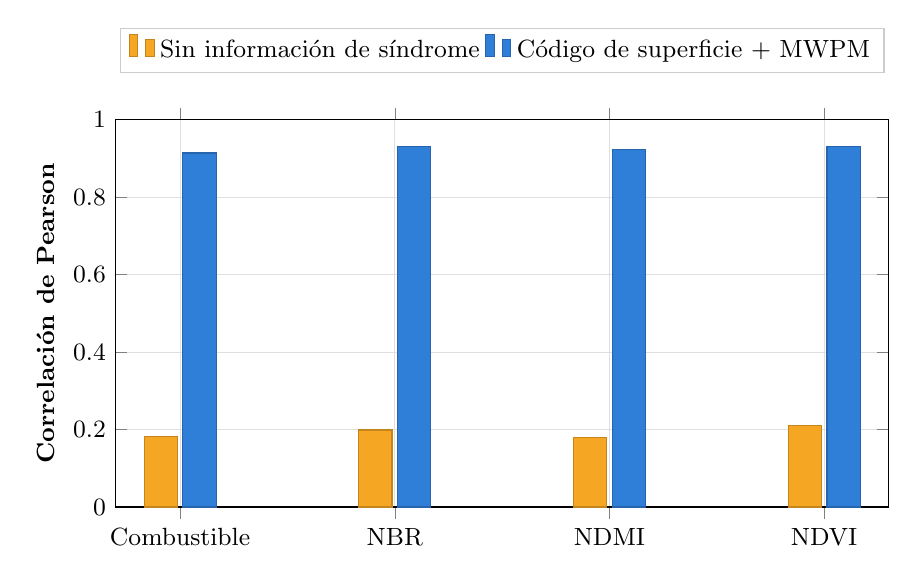
\begin{tikzpicture}
\begin{axis}[
width=0.94\textwidth,height=6.5cm,
ybar,bar width=12pt,ymin=0,ymax=1.0,
symbolic x coords={Combustible,NBR,NDMI,NDVI},xtick=data,
ylabel={Correlación de Pearson},
grid=major,major grid style={draw=gray!25},
legend style={at={(0.5,1.12)},anchor=south,legend columns=2,font=\small,draw=gray!40},
tick label style={font=\small},label style={font=\small\bfseries}
]
\addplot+[fill=channelOrange,draw=channelOrange!80!black] coordinates {(Combustible,0.183)(NBR,0.199)(NDMI,0.180)(NDVI,0.211)};
\addlegendentry{Sin información de síndrome}
\addplot+[fill=mwpmBlue,draw=mwpmBlue!80!black] coordinates {(Combustible,0.914)(NBR,0.931)(NDMI,0.923)(NDVI,0.930)};
\addlegendentry{Código de superficie + MWPM}
\end{axis}
\end{tikzpicture}
\caption{Correlación de Pearson entre productos reconstruidos y originales. MWPM elevó la correlación desde valores inferiores a 0.22 hasta superiores a 0.91 en los cuatro productos espectrales.}
\label{fig:correlacion_espectral}
\end{figure}


\subsection*{Efecto posterior sobre los modelos predictivos}

La evaluación posterior utilizó las instancias principales de CNN, GNN y Transformer, manteniendo fijos sus pesos y umbrales. Los 62 estados con ambas clases se evaluaron bajo condiciones ideal, degradada sin síndrome y reconstruida mediante MWPM. Las métricas se agregaron primero por corrida--semilla y posteriormente entre combinaciones, según el procedimiento descrito en Methods. La variabilidad del entrenamiento se analizó separadamente mediante cinco semillas.

A partir de los RMSE obtenidos para los cuatro productos espectrales,
el factor empírico de atenuación fue
$\widehat{\kappa}\approx0.28$. Por tanto, tras aplicar MWPM permaneció,
como máximo, cerca del $28\%$ del error observado sin síndrome, lo que
equivale a una reducción aproximada del $72\%$. Este indicador resume
la perturbación residual en los productos evaluados y no constituye
una cota general de sensibilidad.

Bajo $p=0.6\%$ y $d=7$, MWPM aumentó el recall de $0.342$ a $0.563$ en el CA, de $0.560$ a $0.704$ en la CNN, de $0.562$ a $0.601$ en la GNN y de $0.359$ a $0.504$ en el Transformer. Las ganancias respectivas fueron $0.221$, $0.144$, $0.039$ y $0.145$, aproximando el desempeño a sus valores ideales ($0.579$, $0.710$, $0.605$ y $0.520$).

El bootstrap jerárquico pareado confirmó mejoras de recall en los
cuatro modelos: CA, $\Delta=0.2209$ (IC95\%:
$[0.1088,\,0.3454]$); CNN, $\Delta=0.1444$
($[0.0653,\,0.2411]$); GNN, $\Delta=0.0384$
($[0.0138,\,0.0647]$); y Transformer, $\Delta=0.1447$
($[0.0803,\,0.1953]$). La exactitud balanceada también mejoró, con
diferencias de $0.1052$, $0.0700$, $0.0166$ y $0.0688$,
respectivamente.

Las mejoras de F1 fueron respaldadas para el CA ($\Delta=0.0357$; IC95\%: $[0.0020,\,0.0776]$) y la CNN ($\Delta=0.0299$; $[0.0006,\,0.0809]$), pero no para la GNN ni el Transformer. Este último presentó además aumentos de AUC ($\Delta=0.0196$; $[0.0027,\,0.0477]$) y AUC-PR ($\Delta=0.0266$; $[0.0005,\,0.0655]$). En conjunto, MWPM produjo efectos más consistentes en recall y exactitud balanceada que en las demás métricas.

\begin{table}[H]
\centering
\caption{Efecto posterior de la protección espectral con ruido físico de 0.6\% y distancia 7. Las métricas son promedios macroagregados sobre 62 estados activos. El diseño cruzó seis corridas primarias con cinco semillas QEC, generando 30 pares corrida--semilla. La inferencia consideró la corrida como unidad primaria de generalización.}
\label{tab:downstream}
\scriptsize
\setlength{\tabcolsep}{3.0pt}
\begin{tabular}{llccccccc}
\toprule
\textbf{Modelo} & \textbf{Condición} & \textbf{F1} & \textbf{IoU} & \textbf{BAcc} & \textbf{Prec.} & \textbf{Recall} & \textbf{AUC} & \textbf{AUC-PR}\\
\midrule
\multirow{3}{*}{CA} & Ideal & 0.227 & 0.137 & 0.772 & 0.146 & 0.579 & 0.971 & 0.253\\
 & Sin inf. de síndrome & 0.190 & 0.115 & 0.659 & 0.141 & 0.342 & 0.969 & 0.247\\
 & MWPM & 0.226 & 0.137 & 0.764 & 0.147 & 0.563 & 0.971 & 0.252\\
\midrule
\multirow{3}{*}{CNN} & Ideal & 0.333 & 0.217 & 0.842 & 0.231 & 0.710 & 0.979 & 0.372\\
 & Sin inf. de síndrome & 0.303 & 0.198 & 0.769 & 0.227 & 0.560 & 0.977 & 0.370\\
 & MWPM & 0.332 & 0.216 & 0.839 & 0.231 & 0.704 & 0.979 & 0.382\\
\midrule
\multirow{3}{*}{GNN} & Ideal & 0.246 & 0.153 & 0.788 & 0.170 & 0.605 & 0.947 & 0.285\\
 & Sin inf. de síndrome & 0.249 & 0.153 & 0.769 & 0.179 & 0.562 & 0.949 & 0.270\\
 & MWPM & 0.244 & 0.151 & 0.786 & 0.168 & 0.601 & 0.948 & 0.282\\
\midrule
\multirow{3}{*}{Transformer} & Ideal & 0.335 & 0.237 & 0.751 & 0.264 & 0.520 & 0.932 & 0.355\\
 & Sin inf. de síndrome & 0.293 & 0.201 & 0.674 & 0.270 & 0.359 & 0.905 & 0.332\\
 & MWPM & 0.327 & 0.228 & 0.743 & 0.258 & 0.504 & 0.925 & 0.359\\
\bottomrule
\end{tabular}
\end{table}

\begin{table}[H]
\centering
\caption{Diferencias pareadas entre MWPM y la condición sin información de síndrome bajo ruido físico de 0.6\% y distancia 7. Los IC95\% se estimaron con 10\,000 réplicas de una aproximación jerárquica pareada al diseño cruzado: se remuestrearon seis corridas y, dentro de cada corrida seleccionada, cinco diferencias asociadas a semillas QEC.}
\label{tab:bootstrap_downstream}
\scriptsize
\setlength{\tabcolsep}{4pt}
\begin{tabular}{lcccc}
\toprule
\textbf{Modelo} & \textbf{$\Delta$F1 [IC95\%]} & \textbf{$\Delta$IoU [IC95\%]} & \textbf{$\Delta$BAcc [IC95\%]} & \textbf{$\Delta$Recall [IC95\%]} \\
\midrule
CA & $0.0357\,[0.0020,\,0.0776]$ & $0.0213\,[0.0002,\,0.0456]$ & $0.1052\,[0.0479,\,0.1677]$ & $0.2209\,[0.1088,\,0.3454]$ \\
CNN & $0.0299\,[0.0006,\,0.0809]$ & $0.0182\,[-0.0022,\,0.0514]$ & $0.0700\,[0.0314,\,0.1190]$ & $0.1444\,[0.0653,\,0.2411]$ \\
GNN & $-0.0054\,[-0.0193,\,0.0145]$ & $-0.0025\,[-0.0144,\,0.0157]$ & $0.0166\,[0.0050,\,0.0294]$ & $0.0384\,[0.0138,\,0.0647]$ \\
Transformer & $0.0338\,[-0.0039,\,0.0844]$ & $0.0271\,[-0.0105,\,0.0796]$ & $0.0688\,[0.0379,\,0.0942]$ & $0.1447\,[0.0803,\,0.1953]$ \\
\bottomrule
\end{tabular}
\end{table}

\begin{figure}[H]
\centering
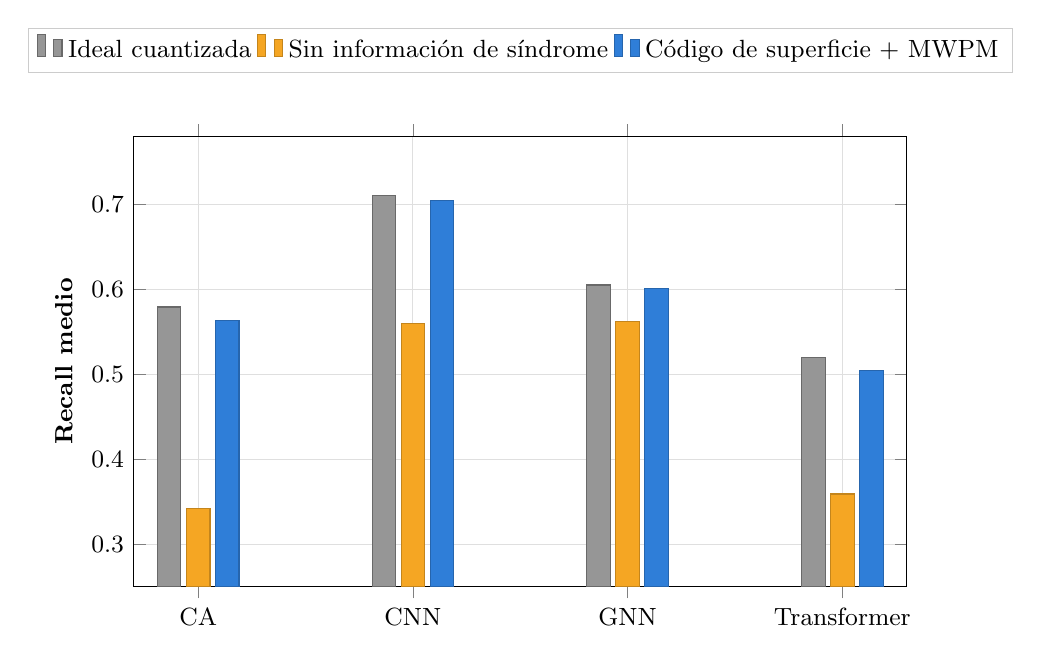
\begin{tikzpicture}
\begin{axis}[
width=0.94\textwidth,height=7.3cm,
ybar,bar width=8.5pt,ymin=0.25,ymax=0.78,
symbolic x coords={CA,CNN,GNN,Transformer},xtick=data,
ylabel={Recall medio},
grid=major,major grid style={draw=gray!25},
legend style={at={(0.5,1.14)},anchor=south,legend columns=3,font=\small,draw=gray!40},
tick label style={font=\small},label style={font=\small\bfseries}
]
\addplot+[fill=idealGray!70,draw=idealGray] coordinates {(CA,0.579)(CNN,0.710)(GNN,0.605)(Transformer,0.520)};
\addlegendentry{Ideal cuantizada}
\addplot+[fill=channelOrange,draw=channelOrange!80!black] coordinates {(CA,0.342)(CNN,0.560)(GNN,0.562)(Transformer,0.359)};
\addlegendentry{Sin información de síndrome}
\addplot+[fill=mwpmBlue,draw=mwpmBlue!80!black] coordinates {(CA,0.563)(CNN,0.704)(GNN,0.601)(Transformer,0.504)};
\addlegendentry{Código de superficie + MWPM}
\end{axis}
\end{tikzpicture}
\caption{Recuperación del recall mediante MWPM a ruido físico de 0.6\% y distancia 7. El efecto fue mayor en CA, CNN y Transformer, y parcial en GNN.}
\label{fig:recall_qec}
\end{figure}

El efecto no fue uniforme para todas las métricas. A distancia 7, MWPM aumentó F1 e IoU en 0.036 y 0.021 para CA, 0.030 y 0.018 para CNN, y 0.034 y 0.027 para Transformer. En GNN, F1 e IoU disminuyeron 0.005 y 0.003, aun cuando recall y balanced accuracy aumentaron. Esta divergencia indica que recuperar valores continuos puede desplazar observaciones alrededor de un umbral fijo. En consecuencia, el aporte del código debe interpretarse mediante el conjunto de métricas, no como una mejora universal de la clasificación.

\subsection*{Aporte comparativo de CNN, GNN y Transformer}

El desempeño de las arquitecturas predictivas se comparó con el
autómata celular para determinar si aportaban capacidad predictiva
adicional respecto de la regla mecanística. El CA alcanzó una elevada
capacidad global para diferenciar las celdas que se incorporaron o no
al frente del incendio, con un AUC de $0.983$. Sin embargo, su
AUC-PR de $0.216$ evidenció un desempeño más limitado sobre la clase
minoritaria, constituida por las nuevas celdas incendiadas.

La CNN presentó el comportamiento más equilibrado entre las métricas
evaluadas y obtuvo los valores más altos de exactitud balanceada
($0.920$), recall ($0.859$), AUC ($0.988$) y AUC-PR ($0.382$).
Estos resultados indican que fue la arquitectura más eficaz para
detectar una mayor proporción de las celdas que efectivamente se
incorporaron al frente, manteniendo al mismo tiempo una elevada
capacidad de discriminación global.

El Transformer alcanzó los mejores valores de F1 ($0.429$), IoU
($0.273$) y precisión ($0.307$). Por tanto, aunque detectó una
proporción menor de celdas incendiadas que la CNN, produjo una
predicción más precisa y con mayor coincidencia espacial respecto del
frente simulado. La GNN, en cambio, obtuvo resultados próximos a los
del CA en F1 e IoU, pero presentó valores inferiores de exactitud
balanceada, recall, AUC y AUC-PR. En consecuencia, bajo la configuración
experimental estudiada, no mostró una ventaja agregada respecto de la
línea base mecanística.

\begin{table}[H]
\centering
\caption{Desempeño microagregado por píxel sobre los 96 estados del mismo conjunto de prueba, con umbrales seleccionados exclusivamente a partir de los datos de entrenamiento.}
\label{tab:modelos}
\scriptsize
\setlength{\tabcolsep}{3.2pt}
\begin{tabular}{lcccccccc}
\toprule
\textbf{Modelo} & \textbf{Umbral} & \textbf{F1} & \textbf{IoU} &
\textbf{BAcc} & \textbf{Prec.} & \textbf{Recall} &
\textbf{AUC} & \textbf{AUC-PR}\\
\midrule
CA          & 0.225 & 0.302 & 0.178 & 0.851 & 0.191 & 0.727 & 0.983 & 0.216\\
CNN         & 0.875 & 0.411 & 0.259 & \textbf{0.920} & 0.270 & \textbf{0.859} & \textbf{0.988} & \textbf{0.382}\\
GNN         & 0.800 & 0.304 & 0.179 & 0.785 & 0.205 & 0.589 & 0.953 & 0.209\\
Transformer & 0.900 & \textbf{0.429} & \textbf{0.273} & 0.851 & \textbf{0.307} & 0.715 & 0.971 & 0.355\\
\bottomrule
\end{tabular}
\end{table}

En comparación con el CA, la CNN mejoró todas las métricas evaluadas.
Sus principales incrementos relativos se observaron en AUC-PR
($76.9\%$), IoU ($45.5\%$) y F1 ($36.1\%$), además de aumentar el
recall en $18.2\%$. Este comportamiento confirma su mayor capacidad
para detectar la clase minoritaria y representar espacialmente el
nuevo frente de propagación.

El Transformer presentó sus mayores mejoras relativas en AUC-PR
($64.4\%$), precisión ($60.7\%$), IoU ($53.4\%$) y F1 ($42.1\%$).
La exactitud balanceada se mantuvo igual a la del CA, mientras que el
recall disminuyó desde $0.727$ hasta $0.715$ y el AUC desde $0.983$
hasta $0.971$. Por tanto, su principal aporte se concentró en producir
predicciones más precisas y con mayor coincidencia espacial, aunque con
una ligera reducción de la sensibilidad y de la discriminación global.

La GNN mostró únicamente mejoras marginales en F1, IoU y precisión.
Estas variaciones no compensaron las reducciones observadas en exactitud
balanceada, recall, AUC y AUC-PR, por lo que no demostró una mejora
global respecto del CA bajo la configuración estudiada. Las diferencias
absolutas se calcularon mediante la ecuación~\ref{eq:delta_metric},
mientras que las variaciones porcentuales se obtuvieron dividiendo cada
diferencia por el resultado correspondiente del CA.

\begin{figure*}[t]
\centering

%================================================
% PANELES EN FORMATO 1 x 3
%================================================
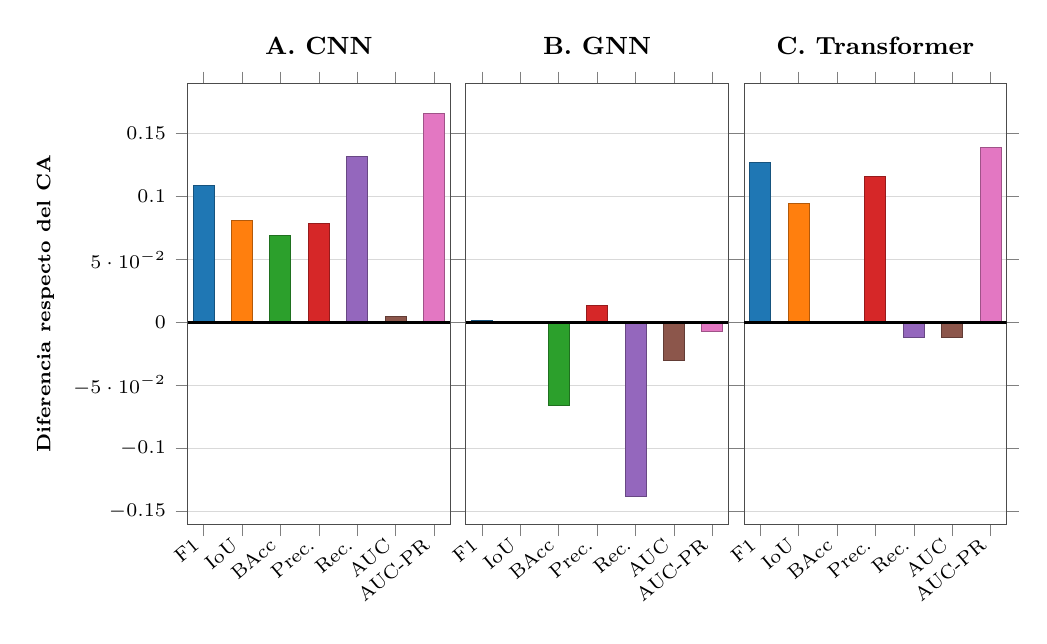
\begin{tikzpicture}

% Comando local para dibujar barras con TikZ nativo. Se evita el uso de
% las claves `bar width` y `bar shift`, incompatibles con algunas versiones
% de PGFPlots incluidas en plantillas editoriales.
\newcommand{\metricbar}[3]{%
    \path[fill=#1,draw=#1!70!black,line width=0.35pt]
      ([xshift=-3.8pt]axis cs:#2,0)
      rectangle
      ([xshift=3.8pt]axis cs:#2,#3);
}

\begin{groupplot}[
    group style={
        group size=3 by 1,
        horizontal sep=2mm,
        y descriptions at=edge left
    },
    width=0.275\textwidth,
    height=5.6cm,
    scale only axis,
    ymin=-0.16,
    ymax=0.19,
    symbolic x coords={
        F1,IoU,BAcc,Prec.,Rec.,AUC,AUC-PR
    },
    xtick={
        F1,IoU,BAcc,Prec.,Rec.,AUC,AUC-PR
    },
    xticklabels={
        F1,IoU,BAcc,Prec.,Rec.,AUC,AUC-PR
    },
    x tick label style={
        rotate=40,
        anchor=east,
        font=\scriptsize
    },
    ytick={
        -0.15,-0.10,-0.05,0,
         0.05,0.10,0.15
    },
    y tick label style={
        font=\scriptsize
    },
    scaled y ticks=false,
    ylabel={Diferencia respecto del CA},
    ylabel style={
        font=\scriptsize\bfseries
    },
    title style={
        font=\small,
        yshift=1pt
    },
    ymajorgrids=true,
    xmajorgrids=false,
    major grid style={
        draw=gray!30,
        line width=0.3pt
    },
    axis line style={
        draw=black!70,
        line width=0.4pt
    },
    enlarge x limits=0.07,
    tick align=outside,
    clip=true
]

%================================================
% PANEL A: CNN
%================================================
\nextgroupplot[
    title={\textbf{A. CNN}}
]
\addplot[draw=none,forget plot] coordinates
  {(F1,0)(IoU,0)(BAcc,0)(Prec.,0)(Rec.,0)(AUC,0)(AUC-PR,0)};

\metricbar{mplBlue}{F1}{0.109}
\metricbar{mplOrange}{IoU}{0.081}
\metricbar{mplGreen}{BAcc}{0.069}
\metricbar{mplRed}{Prec.}{0.079}
\metricbar{mplPurple}{Rec.}{0.132}
\metricbar{mplBrown}{AUC}{0.005}
\metricbar{mplPink}{AUC-PR}{0.166}

\draw[
    black,
    line width=0.9pt
]
    (rel axis cs:0,0.45714)
    --
    (rel axis cs:1,0.45714);

%================================================
% PANEL B: GNN
%================================================
\nextgroupplot[
    title={\textbf{B. GNN}},
    ylabel={}
]
\addplot[draw=none,forget plot] coordinates
  {(F1,0)(IoU,0)(BAcc,0)(Prec.,0)(Rec.,0)(AUC,0)(AUC-PR,0)};

\metricbar{mplBlue}{F1}{0.002}
\metricbar{mplOrange}{IoU}{0.001}
\metricbar{mplGreen}{BAcc}{-0.066}
\metricbar{mplRed}{Prec.}{0.014}
\metricbar{mplPurple}{Rec.}{-0.138}
\metricbar{mplBrown}{AUC}{-0.030}
\metricbar{mplPink}{AUC-PR}{-0.007}

\draw[
    black,
    line width=0.9pt
]
    (rel axis cs:0,0.45714)
    --
    (rel axis cs:1,0.45714);

%================================================
% PANEL C: TRANSFORMER
%================================================
\nextgroupplot[
    title={\textbf{C. Transformer}},
    ylabel={}
]
\addplot[draw=none,forget plot] coordinates
  {(F1,0)(IoU,0)(BAcc,0)(Prec.,0)(Rec.,0)(AUC,0)(AUC-PR,0)};

\metricbar{mplBlue}{F1}{0.127}
\metricbar{mplOrange}{IoU}{0.095}
\metricbar{mplGreen}{BAcc}{0.000}
\metricbar{mplRed}{Prec.}{0.116}
\metricbar{mplPurple}{Rec.}{-0.012}
\metricbar{mplBrown}{AUC}{-0.012}
\metricbar{mplPink}{AUC-PR}{0.139}

\draw[
    black,
    line width=0.9pt
]
    (rel axis cs:0,0.45714)
    --
    (rel axis cs:1,0.45714);

\end{groupplot}

\end{tikzpicture}

%================================================
% LEYENDA CROMÁTICA
%================================================
\vspace{0.7em}

\begingroup
\scriptsize
\setlength{\tabcolsep}{3pt}
\renewcommand{\arraystretch}{1.25}
\begin{tabular}{@{}cl@{\hspace{9pt}}cl@{\hspace{9pt}}cl@{\hspace{9pt}}cl@{}}

\tikz[baseline=-0.5ex]{
    \filldraw[
        fill=mplBlue,
        draw=mplBlue!70!black
    ] (0,0) rectangle (0.22,0.12);
}
& F1

&
\tikz[baseline=-0.5ex]{
    \filldraw[
        fill=mplOrange,
        draw=mplOrange!70!black
    ] (0,0) rectangle (0.22,0.12);
}
& IoU

&
\tikz[baseline=-0.5ex]{
    \filldraw[
        fill=mplGreen,
        draw=mplGreen!70!black
    ] (0,0) rectangle (0.22,0.12);
}
& BAcc

&
\tikz[baseline=-0.5ex]{
    \filldraw[
        fill=mplRed,
        draw=mplRed!70!black
    ] (0,0) rectangle (0.22,0.12);
}
& Prec.\\

\tikz[baseline=-0.5ex]{
    \filldraw[
        fill=mplPurple,
        draw=mplPurple!70!black
    ] (0,0) rectangle (0.22,0.12);
}
& Rec.

&
\tikz[baseline=-0.5ex]{
    \filldraw[
        fill=mplBrown,
        draw=mplBrown!70!black
    ] (0,0) rectangle (0.22,0.12);
}
& AUC

&
\tikz[baseline=-0.5ex]{
    \filldraw[
        fill=mplPink,
        draw=mplPink!70!black
    ] (0,0) rectangle (0.22,0.12);
}
& AUC-PR

&
\tikz[baseline=-0.5ex]{
    \draw[
        black,
        line width=0.9pt
    ] (0,0.06)--(0.30,0.06);
}
& $\Delta=0$

\end{tabular}
\endgroup

\vspace{-0.3em}

\caption{
Diferencias absolutas de CNN, GNN y Transformer respecto del CA.
Los valores positivos indican mejoras y los negativos, reducciones;
la línea negra representa $\Delta=0$. La CNN mostró el desempeño más
equilibrado, el Transformer destacó en F1, IoU y precisión, y la GNN
presentó aportes marginales.}

\label{fig:panel_aporte_modelos_ca}
\end{figure*}

\subsubsection*{Robustez frente a la semilla de entrenamiento}

La CNN, la GNN dirigida y el Transformer se entrenaron con cinco semillas (42--46), manteniendo la misma partición de 14 corridas de entrenamiento y seis de prueba, la configuración de las arquitecturas y un máximo de 20 épocas. El umbral se calibró para cada instancia sobre el conjunto de entrenamiento.

El Transformer presentó el mejor equilibrio y la menor variabilidad, con F1 de $0.438\pm0.010$ (IC95\%: $[0.431,\,0.446]$), IoU de $0.280\pm0.008$ y precisión de $0.310\pm0.013$. La CNN alcanzó el mayor recall ($0.790\pm0.087$) y exactitud balanceada ($0.886\pm0.041$), aunque con mayor variabilidad en F1 ($0.406\pm0.045$). La GNN mostró el desempeño más bajo y la mayor variabilidad del recall, con F1 de $0.267\pm0.034$ y recall de $0.643\pm0.109$. En conjunto, las cinco repeticiones respaldan la estabilidad del Transformer, la mayor sensibilidad pero menor estabilidad de la CNN y el aporte más limitado de la GNN dentro de la configuración evaluada.


\section*{Discussion}

Los resultados responden de manera diferenciada a las dos preguntas de investigación. CNN y Transformer mejoraron respecto del CA nominal, pero con perfiles complementarios: la CNN alcanzó mayor recall y AUC-PR, mientras que el Transformer obtuvo mayor precisión e IoU. Esta comparación considera que las etiquetas proceden de realizaciones estocásticas con un coeficiente de propagación variable, mientras la referencia CA utilizó $\beta=0.30$. Por tanto, las redes aproximaron mejor esa variabilidad que la referencia mecanística nominal, pero no superaron al mecanismo generador en todas sus condiciones. La GNN no mostró una ventaja agregada, posiblemente porque su adyacencia fija, construida con viento de $45^\circ$, limitó la representación de la variabilidad entre corridas.

La evaluación con cinco semillas confirmó la mayor estabilidad del Transformer, con desviaciones estándar de $0.010$ en F1 y $0.008$ en IoU y un umbral constante. La CNN mantuvo un desempeño competitivo, aunque más sensible a la calibración, mientras que la GNN presentó menor desempeño medio y mayor variabilidad relativa del recall. Así, la comparación no depende de una única inicialización, aunque la evaluación causal de QEC mantuvo fijos los pesos y umbrales de las instancias obtenidas en la ejecución principal.

La prevalencia positiva inferior al 1\% explica que el CA alcanzara AUC=0.983, pero solo AUC-PR=0.216. En este contexto, AUC-PR describe mejor la detección del frente minoritario; sus aumentos a 0.382 en CNN y 0.355 en Transformer son más informativos que las pequeñas diferencias de AUC.

El resultado más sólido de la rama cuántica ocurrió antes de la clasificación. Bajo $p=0.6\%$ y $d=7$, MWPM redujo el LER en 93.8\% y reconstruyó los productos espectrales con correlaciones superiores a 0.91, frente a valores inferiores a 0.22 al ignorar los síndromes. El efecto posterior fue más consistente en recall y exactitud balanceada que en F1 o IoU: sus intervalos excluyeron cero en los cuatro modelos, mientras que F1 solo presentó intervalos completamente positivos en CA y CNN. La evidencia respalda, por tanto, una preservación de la sensibilidad frente a nuevas celdas, no una mejora universal de todas las métricas.

El código de superficie tampoco mejoró intrínsecamente los modelos. La intervención modificó exclusivamente las entradas, manteniendo pesos y umbrales. El experimento simula una memoria lógica y su decodificación mediante MWPM; los flujos de fallos se redimensionaron y aplicaron mediante XOR a la carga geoespacial cuantizada. En consecuencia, los resultados representan la transferencia de tasas de fallo derivadas del circuito, no una transmisión cuántica extremo a extremo de la imagen.

La inferencia utilizó una aproximación jerárquica pareada al diseño cruzado. Las seis corridas se remuestrearon como unidades primarias y, dentro de cada corrida seleccionada, se remuestrearon las diferencias asociadas a cinco semillas QEC. Este procedimiento incorpora empíricamente la heterogeneidad entre corridas y la variación Monte Carlo, preserva el pareamiento entre condiciones y evita tratar las 30 combinaciones como incendios independientes. Sus intervalos representan exclusivamente incertidumbre interna de la configuración simulada.

Las limitaciones incluyen una sola escena EuroSAT, una grilla $20\times20$, etiquetas sintéticas, dirección fija de viento, seis corridas primarias, cinco semillas de entrenamiento y un modelo específico de ruido. La referencia sin información de síndrome no representa un canal clásico general, y el estudio no establece una ventaja frente a códigos clásicos. El control de repetición incluido en el notebook utiliza otra carga útil y otro modelo de ruido, por lo que solo ofrece una referencia cualitativa. La generalización requiere múltiples regiones y eventos observados, validación espacial independiente, más corridas y comparaciones clásicas bajo iguales condiciones. Finalmente, aunque NBR fue protegido radiométricamente, evaluar su aporte predictivo exige incorporarlo como entrada y reentrenar las arquitecturas.

\section*{Methods}

\subsection*{Arquitectura del sistema experimental}

El sistema integra preparación geoespacial, simulación CA, protección de productos espectrales mediante QEC y evaluación de CNN, GNN y Transformer (Figura~\ref{fig:pipeline}).

\begin{figure}[htbp]
\centering
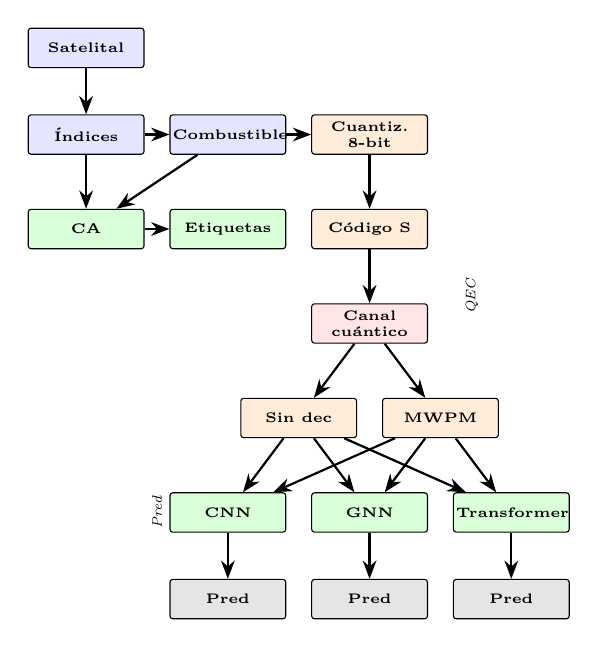
\begin{tikzpicture}[
    block/.style={
        rectangle,
        draw,
        rounded corners=1pt,
        text width=1.4cm,
        text centered,
        minimum height=0.5cm,
        font=\tiny\bfseries,
        fill=gray!10,
        inner sep=1pt
    },
    arrow/.style={thick, -{Stealth}, font=\tiny}
]

% ============================================================
% NODOS
% ============================================================

% Entrada
\node[block, fill=blue!10] (sat) at (0, 0) {Satelital};

% Procesamiento
\node[block, fill=blue!10] (indices) at (0, -1.1) {Índices};
\node[block, fill=blue!10] (fuel) at (1.8, -1.1) {Combustible};

% CA
\node[block, fill=green!15] (ca) at (0, -2.3) {CA};
\node[block, fill=green!15] (labels) at (1.8, -2.3) {Etiquetas};

% QEC
\node[block, fill=orange!15] (quant) at (3.6, -1.1) {Cuantiz. 8-bit};
\node[block, fill=orange!15] (qec) at (3.6, -2.3) {Código S};
\node[block, fill=red!10] (channel) at (3.6, -3.5) {Canal cuántico};
\node[block, fill=orange!15] (bad) at (2.7, -4.7) {Sin dec};
\node[block, fill=orange!15] (good) at (4.5, -4.7) {MWPM};

% Modelos
\node[block, fill=green!15] (cnn)   at (1.8, -5.9) {CNN};
\node[block, fill=green!15] (gnn)   at (3.6, -5.9) {GNN};
\node[block, fill=green!15] (trans) at (5.4, -5.9) {Transformer};

% Salidas
\node[block, fill=gray!20] (out1) at (1.8, -7.0) {Pred};
\node[block, fill=gray!20] (out2) at (3.6, -7.0) {Pred};
\node[block, fill=gray!20] (out3) at (5.4, -7.0) {Pred};

% ============================================================
% CONEXIONES
% ============================================================

% Entrada → índices → combustible
\draw[arrow] (sat) -- (indices);
\draw[arrow] (indices) -- (fuel);

% Índices y combustible → CA → etiquetas
\draw[arrow] (indices) -- (ca);
\draw[arrow] (fuel) -- (ca);
\draw[arrow] (ca) -- (labels);

% Combustible → cuantización → código superficie → canal cuántico
\draw[arrow] (fuel) -- (quant);
\draw[arrow] (quant) -- (qec);
\draw[arrow] (qec) -- (channel);

% Canal → decodificadores
\draw[arrow] (channel) -- (bad);
\draw[arrow] (channel) -- (good);

% Decodificadores → modelos
\draw[arrow] (bad)  -- (cnn);
\draw[arrow] (bad)  -- (gnn);
\draw[arrow] (bad)  -- (trans);
\draw[arrow] (good) -- (cnn);
\draw[arrow] (good) -- (gnn);
\draw[arrow] (good) -- (trans);

% Modelos → predicciones
\draw[arrow] (cnn)   -- (out1);
\draw[arrow] (gnn)   -- (out2);
\draw[arrow] (trans) -- (out3);

% ============================================================
% ETIQUETAS LATERALES
% ============================================================
\node[font=\tiny\itshape, rotate=90] at (4.9, -3.15) {QEC};
\node[font=\tiny\itshape, rotate=90] at (0.9, -5.9) {Pred};

\end{tikzpicture}
\caption{Diagrama de bloques del pipeline experimental. Las cajas azules representan los datos de entrada y productos espectrales; las verdes, el autómata celular y los modelos predictivos; las naranjas, los componentes de corrección de errores cuánticos; y la roja, el canal cuántico con ruido simulado. Las etiquetas laterales indican las dos ramas principales: la rama QEC (corrección de errores cuánticos) y la rama predictiva.}
\label{fig:pipeline}
\end{figure}

\subsection*{Descripción del flujo experimental}

El pipeline contiene una rama predictiva y otra de protección espectral que convergen en la evaluación posterior.

\subsubsection*{Rama izquierda: preparación de datos y simulación de propagación}

Las bandas B04, B08, B11 y B12 del GeoTIFF EuroSAT producen NDVI, NDMI, NBR y combustible. Estos productos alimentan un CA de $20\times20$ celdas y 16 transiciones; las nuevas activaciones del paso siguiente constituyen la variable objetivo.

\subsubsection*{Rama derecha: protección espectral mediante corrección de errores cuánticos}

Los cuatro productos se cuantizan en 8 bits y se someten a patrones de fallo derivados de un código de superficie rotado ($d=3,5,7$) con ruido simulado ($p=0.1\%$ y $0.6\%$). Se comparan un decodificador que ignora los síndromes y MWPM. El experimento transfiere fallos del circuito a una carga digital; no transmite la imagen extremo a extremo mediante qubits.

\subsubsection*{Rama inferior: modelos predictivos}

CNN, GNN y Transformer se entrenan con entradas ideales y se evalúan, sin reajustar pesos ni umbrales, con entradas ideales, degradadas y reconstruidas mediante MWPM. Las métricas principales son F1, IoU, recall, AUC y AUC-PR.


\subsection*{Justificación del diseño}

El diseño prueba si el código de superficie preserva las variables de entrada bajo degradación y limita la transferencia del error hacia modelos clásicos; no atribuye al código una mejora intrínseca del aprendizaje.


\subsection*{Caracterización del experimento}

El experimento utilizó la escena EuroSAT de 13 bandas \texttt{HerbaceousVegetation\_723.tif}, con resolución original de $64\times64$ píxeles, sistema de referencia EPSG:32630 y límites proyectados $(478520.64,6184931.64,479160.70,6185571.69)$. La escena cubrió aproximadamente $640\times640$~m y se remuestreó mediante interpolación bilineal a una grilla computacional de $20\times20$. Se empleó el perfil EuroSAT-13, con bandas roja B04, NIR B08, SWIR1 B11 y SWIR2 B12. Los valores medios observados fueron 0.623 para NDVI, 0.184 para NDMI, 0.483 para NBR y 0.604 para combustible normalizado. La propagación se representó durante 16 transiciones por corrida. Las 14 corridas de entrenamiento generaron 224 estados y las 6 de prueba, 96 estados, sin compartir corridas entre particiones. Entre los estados de prueba, 62 contuvieron ambas clases y 34 no presentaron un nuevo frente. La proporción positiva fue 0.99\% en entrenamiento y 0.83\% en prueba, por lo que se priorizaron F1, IoU, recall y AUC-PR sobre la exactitud simple.

\subsection*{Datos satelitales y productos espectrales}

Se verificó la correspondencia de las 13 bandas del archivo GeoTIFF EuroSAT y se seleccionaron las necesarias para el análisis: B04, correspondiente al rojo visible; B08, al infrarrojo cercano; y B11 y B12, a dos regiones del infrarrojo de onda corta. Estas bandas se utilizaron para calcular los índices espectrales asociados con el estado de la vegetación, su contenido de humedad y las condiciones del combustible.
Los índices fueron calculados como se muestra en las ecuaciones \ref{eq:ndvi}, \ref{eq:ndmi} y \ref{eq:nbr}:
\begin{align}
\mathrm{NDVI}&=\frac{\mathrm{NIR}-\mathrm{Red}}{\mathrm{NIR}+\mathrm{Red}}, \label{eq:ndvi} \\
\mathrm{NDMI}&=\frac{\mathrm{NIR}-\mathrm{SWIR1}}{\mathrm{NIR}+\mathrm{SWIR1}}, \label{eq:ndmi} \\
\mathrm{NBR}&=\frac{\mathrm{NIR}-\mathrm{SWIR2}}{\mathrm{NIR}+\mathrm{SWIR2}}. \label{eq:nbr}
\end{align}
Los productos se normalizaron robustamente entre los percentiles 2 y 98. La vegetación correspondió al NDVI normalizado; la sequedad se definió como uno menos NDMI normalizado; y el combustible se obtuvo a partir de vegetación y sequedad con suavizado gaussiano. Agua, valores inválidos y combustible inferior a 0.10 se trataron como barreras.

\subsection*{Autómata celular y partición experimental}

Cada celda adoptó uno de cuatro estados: combustible no quemado, fuego activo, quemado o barrera. La vecindad de Moore incluyó ocho celdas. La probabilidad de ignición de una celda $i$ se calcula según la ecuación \ref{eq:ca_ignition}:
\begin{equation}
p_i=1-\exp\left[-\beta f_i\sum_{j\in\mathcal{N}_i}I_j
\left(1+w\max(0,\hat{d}_{ji}^{\top}\hat{v})\right)\right], \label{eq:ca_ignition}
\end{equation}
donde $f_i$ es combustible, $I_j$ indica fuego activo, $w$ es intensidad del viento, $\hat{d}_{ji}$ representa la dirección entre celdas, $\hat{v}$ la dirección del viento y $\beta$ la propagación base. Se generaron 20 corridas con semillas y puntos de ignición distintos. La intensidad del viento se muestreó uniformemente entre 0.15 y 0.35, mientras que su dirección permaneció fija en $45^\circ$. El coeficiente de propagación de cada realización varió en $\pm15\%$ alrededor de $\beta=0.30$. Las primeras 14 corridas se utilizaron para entrenamiento y las 6 restantes para prueba. La separación por corridas completas evitó que estados sucesivos de una misma simulación aparecieran en ambos conjuntos.

La entrada de ocho canales incluyó combustible, sequedad, vegetación, fuego activo, superficie quemada, densidad de vecinos activos, intensidad del viento y ángulo normalizado. La etiqueta fue el conjunto de celdas activadas en el paso siguiente.

\subsection*{Arquitecturas predictivas}


Cada arquitectura abordó la propagación desde una perspectiva espacial
diferente. La CNN reconoció patrones locales mediante dos capas
convolucionales con 24 filtros de $3\times3$, seguidas de una proyección
de $1\times1$ para obtener la probabilidad de propagación en cada celda.
El Transformer proyectó los ocho canales de entrada en vectores de
dimensión 24, incorporó posiciones aprendibles para conservar la
ubicación espacial y utilizó una capa codificadora con cuatro cabezas
de atención y dimensión interna 48, permitiendo relacionar distintas
zonas del territorio. Por su parte, la GNN representó cada celda como
un nodo y sus relaciones de vecindad mediante una matriz de adyacencia
dirigida, cuyas conexiones fueron ponderadas según su alineación con
el viento; la información resultante fue procesada mediante tres capas
lineales.

Los tres modelos se entrenaron durante 20 épocas con el optimizador
AdamW, una tasa de aprendizaje de $0.002$, lotes de ocho muestras y una
función de entropía cruzada binaria ponderada para compensar el menor
número de celdas que se incorporaron al frente del incendio. El
autómata celular se utilizó como línea base mecanística nominal y generó sus
estimaciones sin observar el estado futuro, empleando $\beta=0.30$. A diferencia de esta referencia fija, las etiquetas procedieron de realizaciones con coeficientes de propagación variables. Para asegurar una
comparación equitativa, el umbral que maximizó F1 se seleccionó
exclusivamente con los datos de entrenamiento y se aplicó sin
modificaciones al conjunto de prueba.

El desempeño se evaluó mediante F1, IoU, exactitud balanceada,
precisión, recall, AUC y AUC-PR, calculadas con herramientas de
aprendizaje automático reproducibles \cite{pedregosa2011}. El aporte absoluto de cada modelo
respecto del autómata celular se calculó como:

\begin{equation}
\Delta M_k = M_k - M_{\mathrm{CA}},
\label{eq:delta_metric}
\end{equation}

donde $M_k$ corresponde al resultado del modelo evaluado y
$M_{\mathrm{CA}}$ al resultado del autómata celular. Un valor positivo
de $\Delta M_k$ indica una mejora respecto del CA, mientras que un valor
negativo señala un desempeño inferior. El aporte relativo se obtuvo
dividiendo $\Delta M_k$ por $M_{\mathrm{CA}}$, siempre que este último
fuera distinto de cero.


\subsubsection*{Evaluación multisemilla del entrenamiento}

La sensibilidad a la inicialización y al proceso de optimización se
evaluó mediante cinco semillas de entrenamiento:
$\{42,43,44,45,46\}$. Para cada semilla se reinicializaron los
generadores aleatorios de NumPy y PyTorch, los pesos de la arquitectura
y el orden de los lotes. Se conservaron sin cambios la partición por
corridas, las variables de entrada, la configuración arquitectónica,
la tasa de aprendizaje, el tamaño de lote y el máximo de 20 épocas.

Cada instancia se entrenó utilizando 224 estados procedentes de 14
corridas y se evaluó sobre los mismos 96 estados correspondientes a
seis corridas de prueba. El umbral de decisión se calibró
independientemente para cada instancia utilizando exclusivamente la
información de entrenamiento. Para F1, IoU, exactitud balanceada,
precisión y recall se calcularon la media, la desviación estándar y un
intervalo bootstrap del 95\% sobre las cinco semillas. Los intervalos
se utilizaron como una descripción de la variabilidad entre instancias
entrenadas y no como evidencia de generalización territorial.


\subsection*{Código de superficie y comparación pareada}

La protección de la información se simuló mediante circuitos de memoria
$X$ basados en un código de superficie rotado. Se evaluaron distancias
$d\in\{3,5,7\}$ y, para cada distancia, se utilizó un número de rondas
igual a $d$. Una mayor distancia implica distribuir la información
lógica entre más qubits físicos, aumentando la redundancia disponible
para detectar y corregir errores.

El modelo de ruido incluyó cuatro fuentes de error: despolarización
después de las compuertas Clifford, despolarización de los qubits de
datos antes de cada ronda, errores de medición y errores posteriores al
reinicio. Todas estas fuentes fueron parametrizadas mediante
probabilidades físicas de error $p\in\{0.001,0.006\}$, equivalentes a
$0.1\%$ y $0.6\%$, respectivamente. Cada combinación de distancia y
nivel de ruido se ejecutó con $20\,000$ \textit{shots} y cinco semillas
aleatorias independientes.

Se compararon dos condiciones experimentales. En la línea base lógica sin información de síndrome,
los detectores generados por el circuito se ignoraron y
se utilizó como predicción de referencia un observable lógico igual a cero.
En la condición con MWPM, los síndromes se procesaron mediante un
decodificador de emparejamiento perfecto de peso mínimo, construido a
partir del modelo de error de detectores, para identificar la cadena
de errores más probable y estimar el valor lógico corregido.

La comparación se realizó de manera pareada: ambas condiciones
utilizaron exactamente el mismo circuito, nivel de ruido, distancia,
semilla y número de \textit{shots}. La única diferencia experimental
fue el uso o la omisión de la información contenida en los síndromes.
Este diseño permitió atribuir las diferencias observadas al efecto de
utilizar los síndromes mediante MWPM dentro del mismo circuito. La referencia no se interpretó como un canal clásico no protegido. Para $d=3$, $5$ y $7$, los circuitos incluyeron 26, 64 y 118 qubits y 24, 120 y 336 detectores, respectivamente.

\subsection*{Cuantización y reconstrucción espectral}

Cada producto espectral normalizado, con valores $x\in[0,1]$, se
convirtió a una representación digital de 8 bits. Como se indica en la
ecuación~\ref{eq:quantization}, cada valor continuo se asignó a uno de
los 256 niveles enteros comprendidos entre 0 y 255. Posteriormente, el
valor cuantizado se transformó nuevamente al intervalo $[0,1]$ para
obtener su reconstrucción:

\begin{equation}
q(x)=\operatorname{round}(255x),
\qquad
\hat{x}=\frac{q(x)}{255}.
\label{eq:quantization}
\end{equation}

Cada producto espectral de $20\times20$ celdas, cuantizado en 8 bits, generó una carga útil principal de $3\,200$ bits. Para cada producto, semilla y condición experimental se permutó el flujo de $20\,000$ indicadores de fallo lógico y se seleccionaron $3\,200$ posiciones, sin repetir observaciones en la reconstrucción espectral principal. Los patrones resultantes se aplicaron sobre
los bits mediante la operación lógica XOR. Esta operación invierte los
bits afectados por un fallo y permite representar cómo los errores del
circuito degradan los valores espectrales. Después de aplicar los
patrones correspondientes a las condiciones sin información de síndrome y con
MWPM, las secuencias binarias se transformaron nuevamente en valores
numéricos para reconstruir los productos espectrales. El procedimiento transfiere al payload la tasa empírica de fallos lógicos del circuito, pero no representa una transmisión cuántica independiente de cada bit espectral.

La calidad de las reconstrucciones se evaluó mediante el error absoluto
medio (MAE), la raíz del error cuadrático medio (RMSE), la correlación
de Pearson, el índice de similitud estructural (SSIM) \cite{wang2004} y la relación
señal-ruido de pico (PSNR). MAE, RMSE y correlación se calcularon sobre los píxeles válidos; SSIM y PSNR se calcularon sobre la grilla normalizada completa, con rango de datos igual a 1. La contribución de MWPM se calculó de forma
que un valor positivo representara siempre una mejora. Para las métricas
de error se utilizó:

\begin{equation}
\Delta E = E_{\mathrm{sin}}-E_{\mathrm{MWPM}},
\label{eq:delta_error}
\end{equation}

mientras que para las métricas de similitud se empleó:

\begin{equation}
\Delta S = S_{\mathrm{MWPM}}-S_{\mathrm{sin}},
\label{eq:delta_similarity}
\end{equation}

donde los subíndices $\mathrm{sin}$ y $\mathrm{MWPM}$ representan,
respectivamente, las reconstrucciones obtenidas sin información de síndrome y
con decodificación MWPM. De esta manera, $\Delta E>0$ indica una
reducción del error y $\Delta S>0$ señala un aumento de la similitud
respecto del producto espectral original.

\subsection*{Evaluación posterior y análisis estadístico}

Para aislar el efecto de la degradación y reconstrucción espectral, el
análisis posterior a QEC utilizó las instancias obtenidas en la
ejecución principal. En prueba se sustituyeron los canales de combustible, NDMI
y NDVI por sus versiones ideal cuantizada, degradada y corregida,
manteniendo fijos los pesos y los umbrales de esas instancias. El
análisis multisemilla del entrenamiento se realizó separadamente y no
se combinó con el remuestreo jerárquico de corridas y semillas QEC. NBR
no se añadió como entrada porque ello habría requerido modificar y
reentrenar las arquitecturas.

Las métricas discriminativas posteriores a QEC se calcularon en los 62
estados que contenían ambas clases. Para evitar que los pasos sucesivos
de una misma propagación fueran tratados como réplicas independientes,
las métricas se promediaron primero dentro de cada combinación de
corrida de prueba y semilla QEC. De este modo se obtuvieron 30 pares
corrida--semilla, correspondientes al cruce de seis corridas primarias
con las mismas cinco semillas QEC.

La incertidumbre asociada al aporte de MWPM se estimó con 10\,000
réplicas de un bootstrap jerárquico pareado de dos etapas. Primero se
calcularon, para cada corrida $r$ y semilla QEC $s$, las diferencias
entre MWPM y la condición sin información de síndrome:

\begin{equation}
\Delta_{r,s}(M)=M_{\mathrm{MWPM},r,s}-M_{\text{sin información de síndrome},r,s},
\label{eq:delta_bootstrap}
\end{equation}

donde $M$ representa F1, IoU, exactitud balanceada, precisión, recall,
AUC o AUC-PR. En cada réplica se remuestrearon con reemplazo las seis
corridas; dentro de cada corrida seleccionada se remuestrearon con
reemplazo sus cinco valores $\Delta_{r,s}(M)$, y se promediaron los 30
valores resultantes. Los IC95\% son los percentiles 2.5 y 97.5. La
corrida se mantuvo como unidad primaria de generalización, aunque el
segundo nivel incorpora variabilidad entre semillas QEC.

La estructura de dos etapas se justificó porque las cinco semillas QEC
son realizaciones estocásticas repetidas sobre cada una de las mismas
seis corridas y, por tanto, no constituyen unidades territoriales
independientes. Remuestrear únicamente los 30 pares ignoraría su
agrupación por corrida, mientras que promediar previamente las semillas
eliminaría del intervalo la variación Monte Carlo observada dentro de
cada corrida. El esquema jerárquico incorpora empíricamente la heterogeneidad entre corridas y la variación Monte Carlo observada entre semillas QEC, manteniendo la corrida como unidad primaria y el pareamiento entre condiciones. Dado que las mismas semillas se aplicaron a todas las corridas, este remuestreo constituye una aproximación jerárquica al diseño cruzado y sus intervalos se interpretan exclusivamente como incertidumbre interna de la configuración simulada.

Las métricas posteriores que requieren ambas clases se calcularon en 62 estados. En contraste, la comparación general de arquitecturas de la
Tabla~\ref{tab:modelos} utilizó una microagregación de todos los píxeles
de los 96 estados de prueba. Por ello, sus valores no son numéricamente
intercambiables con los promedios macroagregados de la
Tabla~\ref{tab:downstream}.

\subsection*{Cuantificación de la propagación del error}

La relación entre degradación y recuperación se resumió mediante un factor empírico de atenuación del error espectral:

\begin{equation}
\widehat{\kappa} =
\max_{p\in\mathcal{S}}
\frac{
\operatorname{RMSE}\!\left(\mathbf{x}_{\mathrm{MWPM}}^{(p)},\mathbf{x}^{*,(p)}\right)
}{
\operatorname{RMSE}\!\left(\mathbf{x}_{\mathrm{deg}}^{(p)},\mathbf{x}^{*,(p)}\right)
},
\label{eq:kappa}
\end{equation}

donde $\mathcal{S}$ incluye los productos espectrales combustible,
NBR, NDMI y NDVI; $\mathbf{x}^{*,(p)}$ corresponde al producto ideal;
$\mathbf{x}_{\mathrm{deg}}^{(p)}$, a su versión degradada sin información de síndrome; y $\mathbf{x}_{\mathrm{MWPM}}^{(p)}$, a la reconstrucción obtenida mediante MWPM.

Para la condición de ruido físico de $0.6\%$ y distancia $d=7$, los
valores de RMSE obtenidos para los cuatro productos producen
$\widehat{\kappa}\approx0.28$. En consecuencia, dentro de los cuatro productos evaluados, el mayor RMSE corregido correspondió aproximadamente al 28\% de su RMSE degradado, equivalente a una atenuación descriptiva cercana al
$72\%$ respecto de la condición sin
decodificación:

\begin{equation}
1-\widehat{\kappa}\approx0.72.
\label{eq:error_reduction}
\end{equation}

Este factor es una síntesis empírica de las reconstrucciones observadas y no una constante de Lipschitz ni una garantía para entradas o modelos no evaluados. Su correspondencia con la recuperación posterior se examinó directamente mediante las métricas pareadas de las tres condiciones. El análisis respalda la interpretación de que MWPM actúa reduciendo
la degradación de las variables de entrada antes de su procesamiento.
Por tanto, su contribución consiste en preservar la información que
sustenta la predicción, sin modificar los parámetros ni mejorar
intrínsecamente la capacidad de aprendizaje de los modelos.

\section*{Conclusion}

La CNN y el Transformer mostraron aportes complementarios respecto del
autómata celular nominal. La CNN destacó por su mayor capacidad para detectar
las celdas incorporadas al nuevo frente y mejorar el desempeño sobre la
clase minoritaria, mientras que el Transformer presentó mejoras en la
precisión y en la coincidencia espacial entre la propagación predicha y
la simulada. En cambio, la GNN no evidenció una ventaja agregada bajo
la configuración experimental evaluada.

Ante la degradación simulada, el código de superficie decodificado
mediante MWPM preservó sustancialmente la estructura de los productos
NDVI, NDMI, NBR y combustible, alcanzando correlaciones superiores a
$0.91$ respecto de los datos originales, luego de reducir el LER de 38.029\% a 2.367\% en el escenario principal. Esta recuperación redujo la
propagación del error hacia el CA, la CNN, la GNN y el Transformer, y
permitió aproximar su desempeño al obtenido con entradas ideales,
particularmente en la detección de las celdas incendiadas.

En consecuencia, la contribución del código de superficie no debe
interpretarse como una mejora intrínseca de los algoritmos predictivos,
sino como un mecanismo previo de resiliencia informacional que protege
las variables utilizadas para predecir la propagación. No obstante, los
resultados proceden de una escena y de condiciones de ruido simuladas.
La validación con múltiples imágenes satelitales, incendios observados,
configuraciones ambientales diversas, varias semillas de entrenamiento y canales de comunicación
físicamente caracterizados, junto con comparaciones clásicas bajo condiciones equivalentes, constituye el siguiente paso para determinar
la generalización y utilidad operacional del enfoque propuesto.

\section*{Disponibilidad de datos}
El experimento utilizó la escena EuroSAT \texttt{HerbaceousVegetation\_723.tif}. El notebook ejecutado, las semillas, las tablas por corrida--semilla y los archivos CSV que sustentan las figuras y resultados se archivarán en un repositorio público persistente. En la versión de envío, esta declaración deberá completarse con el DOI definitivo de Zenodo: \texttt{[DOI\_ZENODO]}. Hasta la publicación del depósito, los materiales pueden solicitarse al autor de correspondencia.

\section*{Disponibilidad del código}
El código empleado para la extracción espectral, simulación CA, entrenamiento de CNN, GNN y Transformer, generación del código de superficie, decodificación MWPM, bootstrap y análisis multisemilla se encuentra en el notebook \texttt{Cellular Automaton error code}. Antes del envío, la versión archivada deberá incluir instrucciones de ejecución, dependencias, semillas y versiones de software, entre ellas Rasterio 1.5.0 y Stim 1.16.0; su enlace definitivo corresponderá al DOI indicado en la declaración de disponibilidad de datos.

\section*{Agradecimientos}
Los autores agradecen al Centro de Investigación Multidisciplinaria en Tecnologías de Telecomunicaciones (CIMTT) del Departamento de Ingeniería Eléctrica de la Universidad de Santiago de Chile por el apoyo institucional y los recursos computacionales.

\section*{Financiamiento}
Este trabajo fue financiado por la Agencia Nacional de Investigación y Desarrollo (ANID), Chile, mediante el proyecto FONDECYT Regular N.\textsuperscript{o} 1261732 y el proyecto ANID/FIU N.\textsuperscript{o} 137139.

\section*{Contribución de los autores}
Felipe Salgado concibió la investigación, diseñó e implementó el experimento, analizó los resultados y redactó el manuscrito. Ismael Soto supervisó la investigación, contribuyó a la interpretación, revisó críticamente el manuscrito y aprobó su versión final. Todos los autores leyeron y aprobaron el manuscrito.

\section*{Información adicional}
\textbf{Conflicto de intereses.} Los autores declaran no tener conflictos de interés.

\begin{thebibliography}{99}
\bibitem{sanmiguelayanz2023} San-Miguel-Ayanz, J. et al. \textit{Forest Fires in Europe, Middle East and North Africa 2022}. Publications Office of the European Union (2023). doi:10.2760/348120.
\bibitem{godfree2021} Godfree, R. C. et al. Implications of the 2019--2020 megafires for the biogeography and conservation of Australian vegetation. \textit{Nature Communications} \textbf{12}, 1023 (2021).
\bibitem{alexandridis2008} Alexandridis, A., Vakalis, D., Siettos, C. I. \& Bafas, G. V. A cellular automata model for forest fire spread prediction. \textit{Applied Mathematics and Computation} \textbf{204}, 191--201 (2008).
\bibitem{lecun2015} LeCun, Y., Bengio, Y. \& Hinton, G. Deep learning. \textit{Nature} \textbf{521}, 436--444 (2015).
\bibitem{kipf2017} Kipf, T. N. \& Welling, M. Semi-supervised classification with graph convolutional networks. In \textit{International Conference on Learning Representations} (2017).
\bibitem{vaswani2017} Vaswani, A. et al. Attention is all you need. In \textit{Advances in Neural Information Processing Systems} \textbf{30} (2017).
\bibitem{dennis2002} Dennis, E., Kitaev, A., Landahl, A. \& Preskill, J. Topological quantum memory. \textit{Journal of Mathematical Physics} \textbf{43}, 4452--4505 (2002).
\bibitem{fowler2012} Fowler, A. G., Mariantoni, M., Martinis, J. M. \& Cleland, A. N. Surface codes: Towards practical large-scale quantum computation. \textit{Physical Review A} \textbf{86}, 032324 (2012).
\bibitem{edmonds1965} Edmonds, J. Paths, trees, and flowers. \textit{Canadian Journal of Mathematics} \textbf{17}, 449--467 (1965).
\bibitem{higgott2022} Higgott, O. PyMatching: A Python package for decoding quantum codes with minimum-weight perfect matching. \textit{ACM Transactions on Quantum Computing} \textbf{3}, 1--16 (2022).
\bibitem{pedregosa2011} Pedregosa, F. et al. Scikit-learn: Machine Learning in Python. \textit{Journal of Machine Learning Research} \textbf{12}, 2825--2830 (2011).
\bibitem{drusch2012} Drusch, M. et al. Sentinel-2: ESA's optical high-resolution mission for GMES operational services. \textit{Remote Sensing of Environment} \textbf{120}, 25--36 (2012). doi:10.1016/j.rse.2011.11.026.
\bibitem{helber2019} Helber, P., Bischke, B., Dengel, A. \& Borth, D. EuroSAT: A novel dataset and deep learning benchmark for land use and land cover classification. \textit{IEEE Journal of Selected Topics in Applied Earth Observations and Remote Sensing} \textbf{12}, 2217--2226 (2019). doi:10.1109/JSTARS.2019.2918242.
\bibitem{tucker1979} Tucker, C. J. Red and photographic infrared linear combinations for monitoring vegetation. \textit{Remote Sensing of Environment} \textbf{8}, 127--150 (1979). doi:10.1016/0034-4257(79)90013-0.
\bibitem{gao1996} Gao, B.-C. NDWI---A normalized difference water index for remote sensing of vegetation liquid water from space. \textit{Remote Sensing of Environment} \textbf{58}, 257--266 (1996). doi:10.1016/S0034-4257(96)00067-3.
\bibitem{miller2007} Miller, J. D. \& Thode, A. E. Quantifying burn severity in a heterogeneous landscape with a relative version of the delta Normalized Burn Ratio (dNBR). \textit{Remote Sensing of Environment} \textbf{109}, 66--80 (2007). doi:10.1016/j.rse.2006.12.006.
\bibitem{ghali2023} Ghali, R. \& Akhloufi, M. A. Deep learning approaches for wildland fires using satellite remote sensing data: Detection, mapping, and prediction. \textit{Fire} \textbf{6}, 192 (2023). doi:10.3390/fire6050192.
\bibitem{hernandez2007} Hern\'andez Encinas, L., Hoya White, S., Mart\'in del Rey, A. \& Rodr\'iguez S\'anchez, G. Modelling forest fire spread using hexagonal cellular automata. \textit{Applied Mathematical Modelling} \textbf{31}, 1213--1227 (2007). doi:10.1016/j.apm.2006.04.001.
\bibitem{huot2022} Huot, F., Hu, R. L., Goyal, N., Sankar, T., Ihme, M. \& Chen, Y.-F. Next Day Wildfire Spread: A machine learning dataset to predict wildfire spreading from remote-sensing data. \textit{IEEE Transactions on Geoscience and Remote Sensing} \textbf{60}, 1--13 (2022). doi:10.1109/TGRS.2022.3192974.
\bibitem{zhang2023} Zhang, C. et al. WFNet: A hierarchical convolutional neural network for wildfire spread prediction. \textit{Environmental Modelling \& Software} \textbf{170}, 105841 (2023). doi:10.1016/j.envsoft.2023.105841.
\bibitem{jiang2022} Jiang, W. et al. Modeling wildfire spread with an irregular graph network. \textit{Fire} \textbf{5}, 185 (2022). doi:10.3390/fire5060185.
\bibitem{zhou2025} Zhou, Y. et al. Comparative and interpretative analysis of CNN and Transformer models in predicting wildfire spread using remote sensing data. \textit{Journal of Geophysical Research: Machine Learning and Computation} \textbf{2}, e2024JH000409 (2025). doi:10.1029/2024JH000409.
\bibitem{horsman2012} Horsman, C., Fowler, A. G., Devitt, S. \& Van Meter, R. Surface code quantum computing by lattice surgery. \textit{New Journal of Physics} \textbf{14}, 123011 (2012). doi:10.1088/1367-2630/14/12/123011.
\bibitem{paler2023} Paler, A. \& Fowler, A. G. Pipelined correlated minimum weight perfect matching of the surface code. \textit{Quantum} \textbf{7}, 1205 (2023). doi:10.22331/q-2023-12-12-1205.
\bibitem{google2025} Google Quantum AI and Collaborators. Quantum error correction below the surface code threshold. \textit{Nature} \textbf{638}, 920--926 (2025). doi:10.1038/s41586-024-08449-y.
\bibitem{wang2004} Wang, Z., Bovik, A. C., Sheikh, H. R. \& Simoncelli, E. P. Image quality assessment: From error visibility to structural similarity. \textit{IEEE Transactions on Image Processing} \textbf{13}, 600--612 (2004). doi:10.1109/TIP.2003.819861.
\end{thebibliography}

\end{document}
